\documentclass[11pt, a4paper]{article}
\usepackage[utf8x]{inputenc}
\usepackage[sort]{natbib}

\usepackage[spanish]{babel}
\usepackage{enumitem}
\usepackage{graphicx}
\usepackage{float}
\usepackage[linktoc=all]{hyperref}

\usepackage{etoolbox}

\usepackage{amsmath}
\usepackage{amssymb}
\usepackage{array}
\usepackage{gensymb}

\usepackage{fancyhdr}
\usepackage[table]{xcolor}
\usepackage{color}
\usepackage{colortbl}
\definecolor{lightgray}{gray}{0.9}
\setlength{\columnsep}{0.5cm}


%------------------- Dimensiones -------------------
\usepackage{geometry}
 \geometry{a4paper,total={170mm,257mm},left=15mm,right=15mm,top=20mm,}
%----------------------------------------------------

%------------------- Encabezado y Pie de pág -------------------
\pagestyle{fancy}
\fancyhf{}
\lhead{Técnicas Digitales IV}
\rhead{TP2}
\rfoot{Página \thepage}
%----------------------------------------------------


%----------------------------- Documento -----------------------------------------------
\begin{document}
\begin{titlepage}
 \centering
	
\includegraphics[scale=0.80]{Imagenes/LOGO.jpg} \par
 	\vspace{1cm}
 	{\scshape\LARGE Universidad Tecnológica Nacional \par}
 	{\scshape\large Facultad Regional de Córdoba \par}
 	\vspace{1cm}
	{\bfseries \Large Trabajo Práctico De Laboratorio $N^{\circ} 2$\par}
 	\vspace{1.5cm}

	\begin{tabular}{ll}
		Navarro, Facundo		&	63809 	
	\end{tabular}
	
	\vspace{1cm}
	Curso: 6r4 \\
	Grupo $N^{\circ} 5$
 	\vfill
	{\bfseries \Large Técnicas Digitales IV\par}
	
	\vspace{1.5cm}
	Docentes: \par
	Ing. Cayuela, Pablo \par
	Ing. Olmedo, Sergio \par

 	\vfill
	{\large \today\par}
\end{titlepage}
	
	
\tableofcontents
\clearpage

\section{Introducción.}
	En este practico de laboratorio se aborda la generación de video VGA a través de la fpga.  

\section{Desarrollo Teórico.}
	VGA es un estándar de video introducido en los finales de 1980 en IBM, y fue ampliamente utilizado en placas gráficas como así también monitores. 

	

\section{Generador de señal de video.}

	\subsection{Consigna.}
		Diseñar la entidad y arquitectura para generar la señal de vídeo de 640x480 pixel con refresco de pantalla de 60 Hz. Se pide que mediante un pulsador, se seleccione la visualización de las barras en forma horizontal o vertical (similar a la figura \textcolor{blue}{\textbf{\ref{fig:barras}}}). La señal debe ser de 8 barras con los colores primarios generados con la señal de color RGB.

		Se debe visualizar un cuadrado de 1 cm de lado con el color complemento del fondo del mismo y se debe mover unos 2 cm/seg. Al colisionar sobre los bordes de la pantalla, debe cambiar la dirección en forma aleatoria.

	\begin{figure}[H]
		\centering
		
\includegraphics[width=0.6\textwidth]{Imagenes/barras.png}
		\caption{Barras patrón.}
		\label{fig:barras}
	\end{figure} 

	\subsection{Modificaciones.}
		Se agregaron las siguientes modificaciones:
		\begin{itemize}
			\item Resolución de 1280x1040x60Hz.
			\item Pelota redonda.
			\item Switch para detener imagen.
		\end{itemize}

	\subsection{Desarrollo.}
		\subsubsection{Estructura del proyecto}
		El proyecto fue desarrollado en el SW Vivado 2019.2.1, ya que se utilizo la plataforma de entrenamiento de Digilent Basys3.

		\begin{figure}[H]
			\centering
			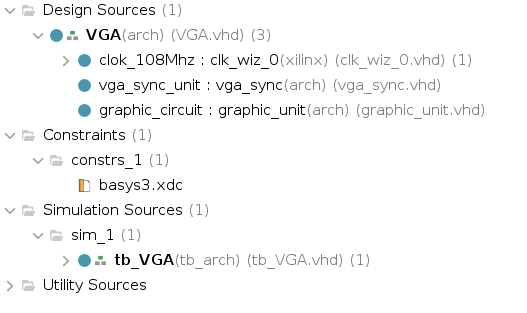
\includegraphics[width=0.5\textwidth]{Imagenes/estructura.png}
			\caption{Árbol del proyecto}
			\label{fig:proyecto_vivado}
		\end{figure} 
		
		\subsection{Multimedia.}
		Se adjunta un dos links de unos vídeos demostrativos: 
		\begin{itemize}
			\item Presentación: \url{https://youtu.be/9nZTGVpQUsM}
			\item Demo: \url{https://youtu.be/1LScYSxSe5s}

\end{document}
